%!TEX TS-program = xelatex 
%!TEX TS-options = -output-driver="xdvipdfmx -q -E"
%!TEX encoding = UTF-8 Unicode
%
%  seminar_1
%
%  Created by Mark Eli Kalderon on 2010-01-17.
%

\documentclass[11pt]{article} 

% Definitions
\newcommand\myauthor{Mark Eli Kalderon} 
\newcommand\mytitle{Empiricism and the Philosophy of Mind}
\newcommand\mysubtitle{Parts III and IV}

% Packages
\usepackage{url}
\usepackage{txfonts}
\usepackage{color}
\definecolor{myblue}{rgb}{0.8,0.8,1}

% Define discussion environment
\makeatletter\newenvironment{discussion}{%
   \noindent\begin{lrbox}{\@tempboxa}\begin{minipage}{\columnwidth}\setlength{\parindent}{1em}}{\end{minipage}\end{lrbox}%
   \colorbox{myblue}{\usebox{\@tempboxa}}
}\makeatother

% XeTeX
\usepackage[cm-default]{fontspec}
\usepackage{xltxtra,xunicode}
\defaultfontfeatures{Scale=MatchLowercase,Mapping=tex-text}
\setmainfont{Palatino}
\setmonofont{Inconsolata}

% Title Information
\title{\mytitle\\
\mysubtitle}
\author{\myauthor} 
\date{} % Leave blank for no date, comment out for most recent date

% PDF Stuff
\usepackage[plainpages=false, pdfpagelabels, bookmarksnumbered, backref, pdftitle={\mytitle}, pagebackref, pdfauthor={\myauthor}, xetex, colorlinks=true, citecolor=gray, linkcolor=gray, urlcolor=gray]{hyperref}

%%% BEGIN DOCUMENT
\begin{document}

% Title Page
\maketitle

% Layout Settings
\setlength{\parindent}{1em}

% Main Content

\begin{figure}[htbp]
	\centering
		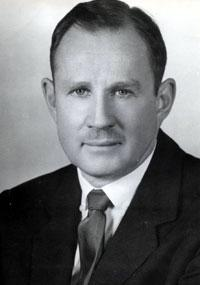
\includegraphics[scale=0.5]{../graphics/sellars.jpeg}
	\caption{Wilfrid Sellars}
	\label{fig:sellars}
\end{figure}

\section{The Logic of Looks} % (fold)
\label{sec:the_logic_of_looks}

\textbf{Section 10}: Sellars has provided (§7) a diagnosis for why the classical sense datum theorist is committed to the inconsistent triad (§6) in terms of their ``crossbreeding of two ideas'':
\begin{enumerate}
    \item The idea that there are certain inner episodes---e.g. sensations of red or of C\# which can occur to human beings (and brutes) without any prior process of learning or concept formation; and without which it would \emph{in some sense} be impossible to \emph{see}, for example, that the facing surface of a physical object is red and triangular, or \emph{hear} that a certain physical sound is C\#.
    \item The idea that there are certain inner episodes which are the non-inferential knowings that certain items are, for example, red or C\#; and that these episodes are the necessary conditions of empirical knowledge as providing evidence for all other empirical propositions.
\end{enumerate}
A full assessment of this diagnosis would involve, inter alia, the development, in light of critical examination, of each, and an inquiry as to how and to what extent these critically developed ideas may be coherently combined. 

One salient feature that would need examination is the idea of an inner episode. Logical positivists deny that there are inner episodes to which subjects have privileged access, since being private, their presence is not subject to public verification. They thus oppose the notion of an inner episode as it figures in the first of the two crossbred ideas. And Wittgensteinians deny that knowledge of inner episodes could be premises on which empirical knowledge rests on a foundation, since inner episodes are private, and the net of rational discourse is public. Whatever the merits of these worries, they couldn't be the heart of the Myth of the Given, since the Myth of the Given can arise in a form that doesn't involve inner episodes:
\begin{quote}
    \ldots\ they have no defense against the myth in the form of givenness of such facts as taht \emph{physical object x looks red to person S at time t}, or that \emph{there looks to person S at time to to be a red physical object over there}.
\end{quote}
This sets the negative agenda of Part III, \emph{The Logic of Looks}. Whereas Parts I \& II are concerned with the Myth of the Given as it arises in the context of classical sense datum theory, Part III will be concerned with the given as it arises in the context of the theory of appearing. 

% section the_logic_of_looks (end)

\section{Explaining Looks} % (fold)
\label{sec:explaining_looks}



% section explaining_looks (end)

\end{document}